% Auto-generated by scripts/benchmark_timing_figure.py -- do not edit by hand.
% Juliet scan time per CWE (parallelism- and corpus-size-independent), v0.3.25-v0.4.45.
\begin{figure}[t]
\centering
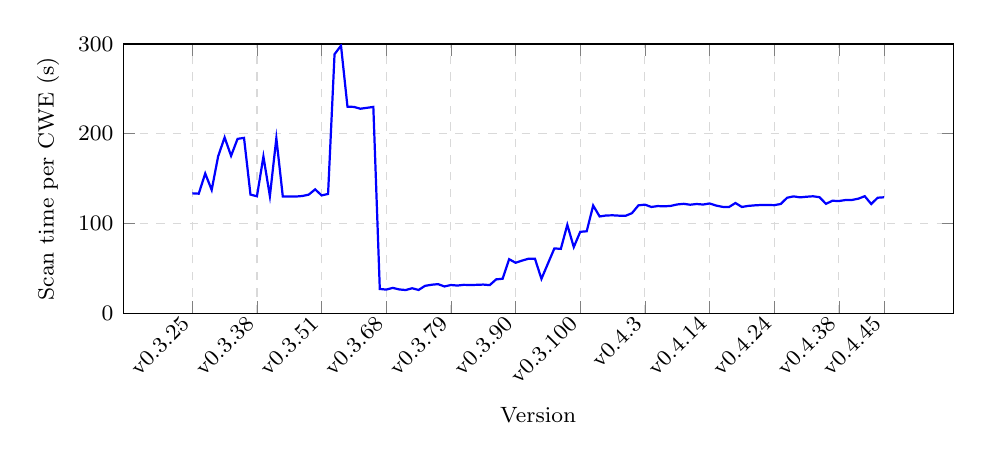
\begin{tikzpicture}
\begin{axis}[
    width=\columnwidth,
    height=5cm,
    xlabel={Version},
    ylabel={Scan time per CWE (s)},
    ymin=0, ymax=300,
    xtick={1, 11, 21, 31, 41, 51, 61, 71, 81, 91, 101, 108},
    xticklabels={v0.3.25, v0.3.38, v0.3.51, v0.3.68, v0.3.79, v0.3.90, v0.3.100, v0.4.3, v0.4.14, v0.4.24, v0.4.38, v0.4.45},
    xticklabel style={rotate=45, anchor=east, font=\footnotesize},
    ylabel style={font=\footnotesize},
    xlabel style={font=\footnotesize},
    tick label style={font=\footnotesize},
    grid=major,
    grid style={dashed, gray!30},
]
\addplot[color=blue, thick, mark=none] coordinates {
    (1, 133.6) (2, 133.2) (3, 155.7) (4, 137.4) (5, 174.9) (6, 195.9) (7, 175.4) (8, 194.3) (9, 195.4) (10, 132.2) (11, 130.3) (12, 174.6) (13, 130.5) (14, 195.0) (15, 130.0) (16, 130.0) (17, 130.0) (18, 130.6) (19, 132.1) (20, 138.0) (21, 131.3) (22, 132.9) (23, 288.6) (24, 298.2) (25, 230.2) (26, 229.9) (27, 227.9) (28, 228.9) (29, 229.9) (30, 27.0) (31, 26.3) (32, 28.2) (33, 26.5) (34, 25.8) (35, 27.8) (36, 25.9) (37, 30.5) (38, 31.7) (39, 32.4) (40, 29.8) (41, 31.4) (42, 30.8) (43, 31.6) (44, 31.4) (45, 31.6) (46, 31.9) (47, 31.3) (48, 37.7) (49, 38.4) (50, 60.2) (51, 56.2) (52, 58.6) (53, 60.7) (54, 60.6) (55, 38.3) (56, 55.3) (57, 72.2) (58, 71.7) (59, 98.5) (60, 73.7) (61, 90.7) (62, 91.3) (63, 120.0) (64, 107.8) (65, 108.9) (66, 109.1) (67, 108.7) (68, 108.5) (69, 111.5) (70, 120.2) (71, 121.0) (72, 118.4) (73, 119.4) (74, 119.1) (75, 119.6) (76, 121.2) (77, 121.9) (78, 120.9) (79, 121.7) (80, 121.1) (81, 122.3) (82, 120.0) (83, 118.5) (84, 118.3) (85, 122.8) (86, 118.4) (87, 119.6) (88, 120.2) (89, 120.6) (90, 120.6) (91, 120.4) (92, 121.7) (93, 128.7) (94, 130.2) (95, 129.1) (96, 129.8) (97, 130.3) (98, 129.3) (99, 121.9) (100, 125.3) (101, 125.0) (102, 126.1) (103, 126.2) (104, 127.6) (105, 130.4) (106, 121.7) (107, 128.7) (108, 129.2)
};
\end{axis}
\end{tikzpicture}
\caption{Juliet scan time per CWE across 108 released versions
(v0.3.25--v0.4.45). The metric is the summed
per-CWE \texttt{sqc} analysis time divided by the number of CWEs scanned,
making it independent of both parallelism (\texttt{--jobs}) and corpus growth
(68--74 CWEs). The sharp drop at v0.3.67 is a single perf optimization
($\approx$8$\times$); the subsequent climb is the cost of added
inter-procedural analysis, which still settles below the v0.3.5x peak.}
\label{fig:scan-time}
\end{figure}
